\subsection*{Problema 21}

\textbf{Enunciado:} \\
Calcular la integral indefinida:
\begin{equation*}
\int \dfrac{\cos x \, dx}{\cos^2 x + 1}
\end{equation*}

\textbf{Solución:} \\
De acuerdo con las indicaciones, utilizamos la identidad trigonométrica fundamental en el denominador:
\begin{equation*}
\cos^2 x = 1 - \sin^2 x
\end{equation*}

Sustituimos esta expresión en la integral original:
\begin{align*}
I &= \int \dfrac{\cos x \, dx}{(1 - \sin^2 x) + 1} \\
  &= \int \dfrac{\cos x \, dx}{2 - \sin^2 x}
\end{align*}

Realizamos el cambio de variable sugerido:
\begin{equation*}
u = \sin x, \quad du = \cos x \, dx
\end{equation*}

Sustituyendo en la integral en términos de $u$:
\begin{equation*}
I = \int \dfrac{du}{2 - u^2}
\end{equation*}

Reescribimos el denominador para aplicar la fórmula de integración estándar para fracciones parciales o funciones inversas:
\begin{equation*}
I = \int \dfrac{du}{(\sqrt{2})^2 - u^2}
\end{equation*}

Recordando la fórmula de integración:
\begin{equation*}
\int \dfrac{du}{a^2 - u^2} = \dfrac{1}{2a} \ln \left| \dfrac{a + u}{a - u} \right| + C
\end{equation*}

Para nuestro caso, $a = \sqrt{2}$:
\begin{equation*}
I = \dfrac{1}{2\sqrt{2}} \ln \left| \dfrac{\sqrt{2} + u}{\sqrt{2} - u} \right| + C
\end{equation*}

Reemplazando nuevamente $u = \sin x$:
\begin{equation*}
I = \dfrac{1}{2\sqrt{2}} \ln \left| \dfrac{\sqrt{2} + \sin x}{\sqrt{2} - \sin x} \right| + C
\end{equation*}

El resultado final de la integral es:
\begin{equation*}
\int \dfrac{\cos x \, dx}{\cos^2 x + 1} = \dfrac{\sqrt{2}}{4} \ln \left| \dfrac{\sqrt{2} + \sin x}{\sqrt{2} - \sin x} \right| + C
\end{equation*}

\begin{figure}[H]
	\centering
	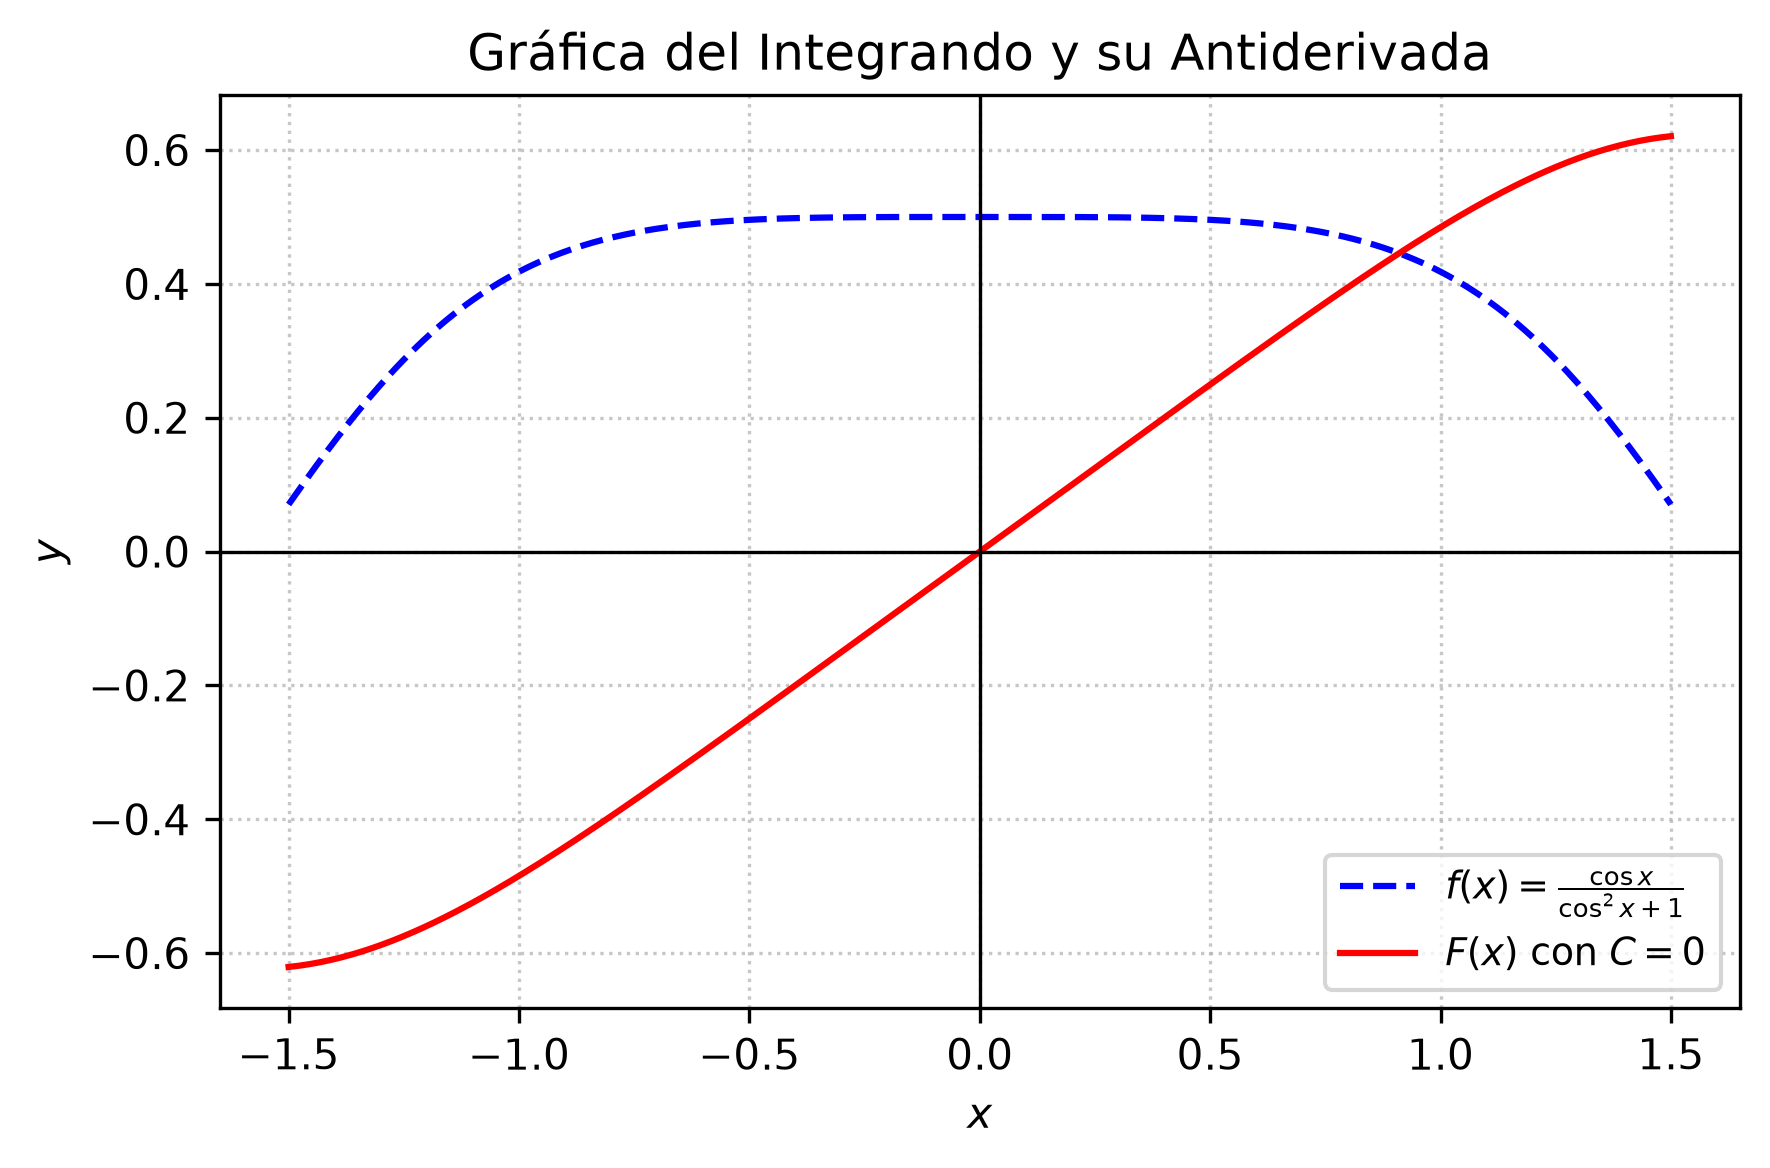
\includegraphics[width=\columnwidth]{semana_04/graficas/SEM04_P21_grafica.png}
	\caption{Representación gráfica de $f(x)$ y su antiderivada $F(x)$ evaluada para la constante de integración $C = 0$ (Problema 21).}
	\label{fig:problema21}
\end{figure}
